\documentclass{beamer}
\usetheme{Singapore}
%\setbeamercolor{structure}{fg=red}
\usepackage{upgreek}
\usepackage{color}
%\def\magyarOptions{hyphenation=huhyphn}
%\usepackage{ae,aecompl}
%\usepackage[T1]{fontenc}
\usepackage[utf8]{inputenc}
%\usepackage[hungarian]{babel}
\usepackage{gensymb}
\usepackage{pgfplots}
\usepackage{pst-plot}
\usepackage{tikz}
\usepgfplotslibrary{external}
\tikzexternalize
\usepackage[version=3]{mhchem}

\normalfont
\title{Recent Advances in Potentiometric Scanning Electrochemical Microscopy}
\subtitle{9$^{th}$ Workshop on Scanning Electrochemical Microscopy and Related Techniques, Warsaw}
\author
{\underline{András Kiss}, Géza Nagy\\}


\institute
{
  %\inst{1}%
  Department of General and Physical Chemistry\\
  University of Pécs, Hungary\\
  \hfill \\

  \includegraphics[width=0.14\textwidth]{pte_logo.eps}\\
  August 16, 2017
}

\date[]

\begin{document}
\frame{\titlepage}  


\begin{frame}
	\centering
	\includegraphics[width=0.6\textwidth]{secm.eps}
	\frametitle{Potentiometric SECM}
\end{frame}


\begin{frame}
	\frametitle{The problem with potentiometric SECM} 
	\framesubtitle{Distortion at high scan rate}
	\centering
\quad\quad\quad\quad\quad\quad Slow \hfill Fast \quad\quad\quad\quad\quad\quad\quad

	\includegraphics[trim = 10mm 30mm 0mm 20mm, clip, width=0.4\textwidth, angle=-90]{real.eps}\hfill\includegraphics[trim = 10mm 30mm 0mm 20mm, clip, width=0.4\textwidth, angle=-90]{fastcomb_sim.eps}
\end{frame}

\begin{frame}
\frametitle{Why is the image distorted?}
\framesubtitle{Possible contributors to the lag}
\centering
\includegraphics[width=0.8\textwidth]{npp.eps}
\end{frame}

\begin{frame}
	\frametitle{Why is the image distorted?}
	\framesubtitle{The RC time constant} 
	\centering
	\includegraphics[width=1\textwidth]{RC.eps}
	\vfill
	The time that is required to charge \\ the capacitor by $\approx 63\%$ $(1-1/e)$.	
	\vfill
	$\tau = R \cdot C$
	
	$R = 5 $ G$\ohm$
	
	$C = 500 $ pF
	
	\textbf{\textcolor{white!100}{\colorbox{red!100}{$\tau = 2.5 $ s}}}

	%\includegraphics[width=0.6\textwidth, angle=-90]{meander_sim.eps}
\end{frame}

\begin{frame}
	\frametitle{Distortion of potentiometric imaging} 
	\framesubtitle{In the case of a linescan} 
	\centering
	\includegraphics[width=0.8\textwidth]{distortion2.eps}
\end{frame}

\begin{frame}
	\centering
	\frametitle{Imaging distortion}
	\framesubtitle{Using the meander algorithm}
	\includegraphics[width=0.4\textwidth, angle=-90]{meander.eps}
\end{frame}




\begin{frame}
	\frametitle{Why is it so important to complete the scan quickly?}
	\framesubtitle{Example: corrosion of a magnesium alloy}
	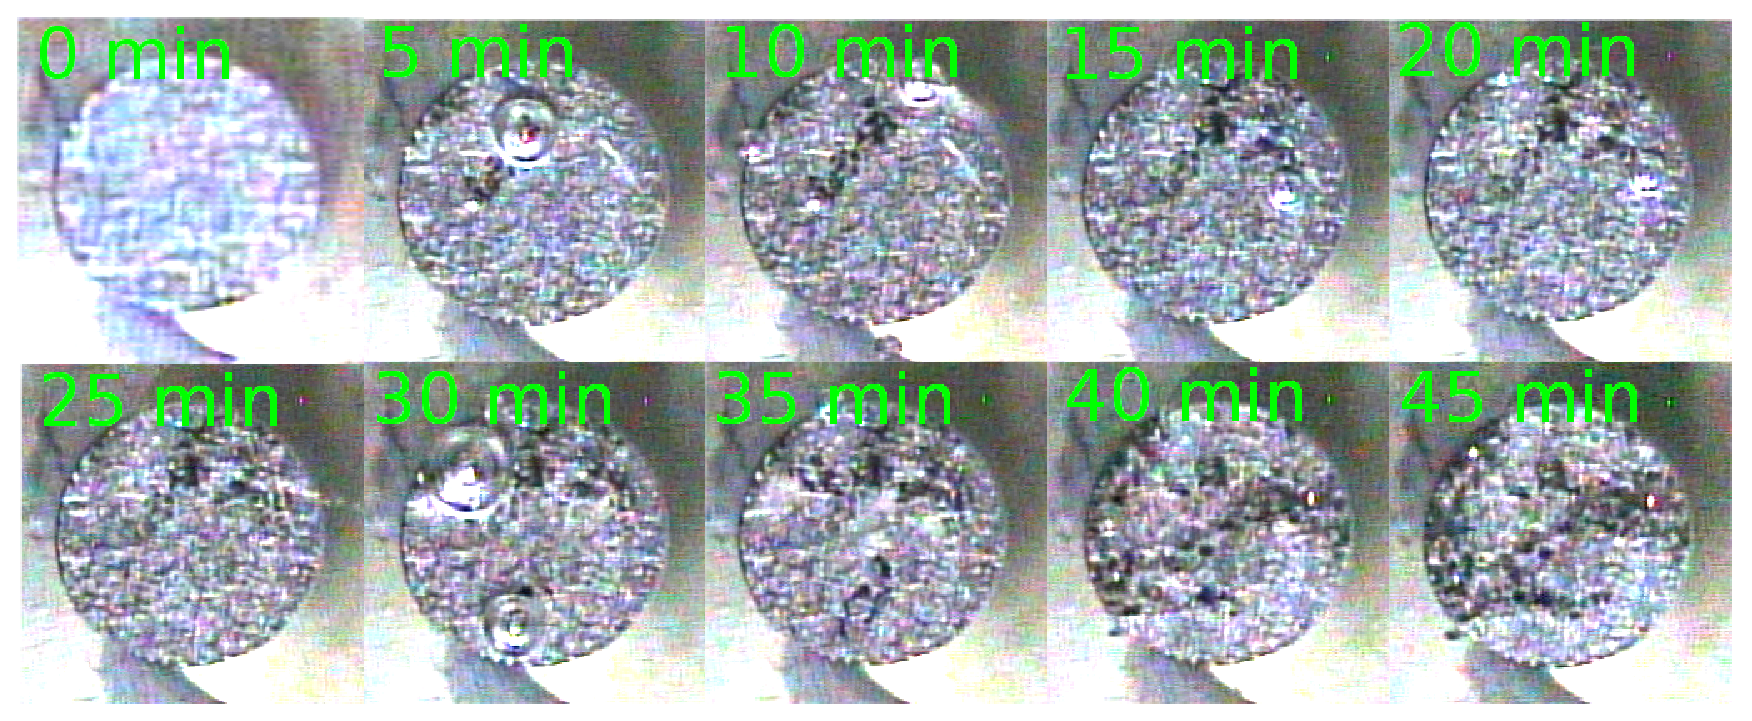
\includegraphics[width=1\textwidth]{timelapse.eps}\\
\centering
Corrosion of the AZ63 magnesium-aluminium-zinc alloy.
%Location of the anodic and cathodic spots change quickly. High-speed scanning is required to complete the scan before the studied system changes.
\end{frame} 

\begin{frame}
\frametitle{Trade-off triangle of potentiometric SECM}
\framesubtitle{Compromise between the three desired competing properties}
\begin{center}
\includegraphics[width=0.5\textwidth]{trade-off.eps}
\end{center}
\end{frame}

\begin{frame}[plain]
\centering
Solution \#1:
Solid contact micropipettes as SECM probes.
\end{frame}

\begin{frame}
\frametitle{Liquid vs. solid contact micropipettes}
\framesubtitle{Comparison of construction}
\begin{center}
\quad\quad\quad\quad Liquid contact \hfill Solid contact \quad\quad\quad\quad

\includegraphics[width=0.9\textwidth]{liquid_solid.jpg}
\end{center}
\end{frame}


\begin{frame}
	\frametitle{Application in corrosion science: galvanic corrosion of Mg} 
	%\framesubtitle{Results}
	\centering
	\quad\quad\quad\quad Liquid contact \hfill Solid contact \quad\quad\quad\quad\quad

	\includegraphics[trim = 10mm 30mm 0mm 20mm, clip, width=0.4\textwidth, angle=-90]{liquid_coupled.eps}\includegraphics[trim = 10mm 30mm 0mm 20mm, clip, width=0.4\textwidth, angle=-90]{solid_coupled.eps}
\end{frame}



\begin{frame} [plain]
\centering
Solution \#2:
Optimizing scanning patterns and algorithms.
\end{frame}

\begin{frame}
	\frametitle{New SECM scanning patterns based on the polar-coordinate system}
	\centering	
	\includegraphics[width=0.7\textwidth]{cartesian_vs_polar.eps}
	
	\vfill
\end{frame}

\begin{frame}
	\centering
	\frametitle{Confirmation with experimental SECM scans}
	\framesubtitle{Recorded using the antimony microelectrode}
	\quad\quad\quad\quad\quad 440 seconds \hfill 340 seconds \quad\quad\quad\quad\quad\quad


	\includegraphics[width=0.3\textwidth, angle=-90]{meander.eps}\includegraphics[width=0.3\textwidth, angle=-90]{arc.eps}\\
	\vfill
	Scans are completed almost 2 times faster,\\ images have almost 10 times less distortion.
\end{frame}

\begin{frame}[plain]
\centering
Solution \#3: Signal processing.
\end{frame}

\begin{frame}
\frametitle{The convolution function of the distortion}
\centering	
\includegraphics[width=1\textwidth]{t.eps}\\
\vfill
$E_{cell}(t) = E_{cell}(\infty) + [E_{cell}(0) - E_{cell}(\infty)]e^{-t/\tau}$\\
\vfill
%$E_{cell}(\infty)	= \frac {\displaystyle [E_{cell}(t) - E_{cell}(0)]e^{-t/RC}}	{\displaystyle 1 - e^{-t/RC}}$
\end{frame}

\begin{frame}
\frametitle{Convolution and deconvolution}
\centering
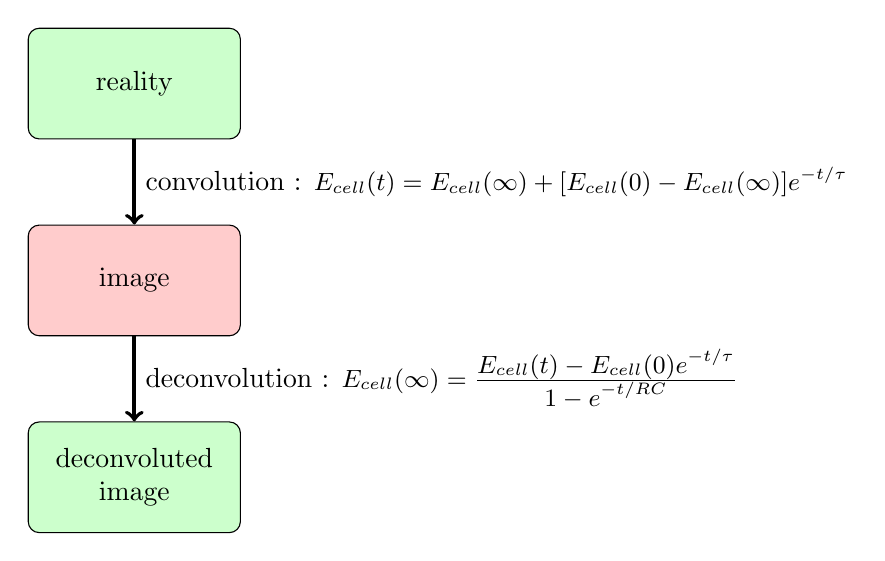
\begin{tikzpicture}[node distance = 2.5cm, auto]
\node [rectangle, draw, fill=green!20,text width=7em, text centered, rounded corners, minimum height=4em] (reality) {reality};
\node [rectangle, below of=reality, draw, fill=red!20,text width=7em, text centered, rounded corners, minimum height=4em] (measurement) {image};
\node [rectangle, below of=measurement, draw, fill=green!20,text width=7em, text centered, rounded corners, minimum height=4em] (image) {deconvoluted\\ image};

\draw [line width=0.5mm, ->] (reality) -- (measurement) node [pos=.5, right] (TextNode) {convolution : \small $E_{cell}(t) = E_{cell}(\infty) + [E_{cell}(0) - E_{cell}(\infty)]e^{-t/\tau}$};
\draw [line width=0.5mm, ->] (measurement) -- (image) node [pos=.5, right] (TextNode) {deconvolution : \small $E_{cell}(\infty)      = \frac {\displaystyle E_{cell}(t) - E_{cell}(0)e^{-t/\tau}}    {\displaystyle 1 - e^{-t/RC}}$};


\end{tikzpicture}
\end{frame}

\begin{frame}
\frametitle{Demonstartion with a model system}
\framesubtitle{Experimental setup}
\begin{center}
\includegraphics[width=0.9\textwidth]{model.eps}
\end{center}
\end{frame}

\begin{frame}
	\frametitle{Deconvolution of potentiometric SECM images}
	\framesubtitle{Recorded using the antimony microelectrode following the meander algorithm}
\centering

\def\s{0.15}

\begin{columns}[T] % align columns

\begin{column}{.2\textwidth}
\begin{minipage}[c][0.75\textheight][c]{\linewidth}
\centering
%raw\\
%images
\end{minipage}
\end{column}%
\hfill%
\begin{column}{.2\textwidth}
\centering
\includegraphics[trim = 10mm 30mm 0mm 10mm, clip, width=0.8\textwidth, angle=-90]{13121313.eps}\\
\includegraphics[trim = 10mm 30mm 0mm 10mm, clip, width=0.8\textwidth, angle=-90]{13121314.eps}\\
\includegraphics[trim = 10mm 30mm 0mm 10mm, clip, width=0.8\textwidth, angle=-90]{13121315.eps}\\
\includegraphics[trim = 10mm 30mm 0mm 10mm, clip, width=0.8\textwidth, angle=-90]{13121316.eps}\\
\end{column}%
\begin{column}{.2\textwidth}
\begin{minipage}[c][0.7\textheight][c]{\linewidth}
\centering
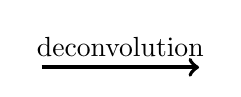
\begin{tikzpicture}
\draw [line width=0.5mm,->] (0,0) -- (2,0) node [pos=.5, above] (TextNode) {deconvolution};
\end{tikzpicture}
\end{minipage}
\end{column}%
\begin{column}{.2\textwidth}
\centering
\includegraphics[trim = 10mm 30mm 0mm 10mm, clip, width=0.8\textwidth, angle=-90]{13121313_deconvoluted.eps}\\
\includegraphics[trim = 10mm 30mm 0mm 10mm, clip, width=0.8\textwidth, angle=-90]{13121314_deconvoluted.eps}\\
\includegraphics[trim = 10mm 30mm 0mm 10mm, clip, width=0.8\textwidth, angle=-90]{13121315_deconvoluted.eps}\\
\includegraphics[trim = 10mm 30mm 0mm 10mm, clip, width=0.8\textwidth, angle=-90]{13121316_deconvoluted.eps}\\
\end{column}%
\begin{column}{.2\textwidth}
\begin{minipage}[c][0.75\textheight][c]{\linewidth}
\centering
%deconvoluted\\
%images
\end{minipage}
\end{column}%
\end{columns}
\end{frame}

\begin{frame}
\frametitle{Deconvolution of potentiometric SECM images}
\framesubtitle{Experimental setup}
\begin{center}
\includegraphics[width=0.9\textwidth]{setup.eps}
\end{center}
\end{frame}


\begin{frame}
\begin{center}
\frametitle{Deconvolution of potentiometric SECM images}
\framesubtitle{Recorded using the magnesium ISME following the meander algorithm}
\includegraphics[width=0.6\textwidth]{mg_2d.pdf}
\end{center}
\end{frame}

\begin{frame}
\frametitle{Practical example: corroding carbon steel sample}
\framesubtitle{Scanned with an antimony microelectrode}
\begin{figure}
\centering
%top left bottom right
\includegraphics[trim = 10mm 30mm 0mm 10mm, clip, width=0.3\textwidth, angle=-90]{16012906.eps}\includegraphics[trim = 10mm 30mm 0mm 10mm, clip, width=0.3\textwidth, angle=-90]{16012906_deconvoluted.eps}

\includegraphics[width=0.24\textwidth]{cs_cut.jpg}

%\caption[Raw, and deconvoluted SECM image and microphoto of a corroding carbon-steel sample polarized anodically.]{Raw (A), and deconvoluted (B) SECM image and microphoto (C) of a corroding carbon-steel sample polarized anodically with a current density of 10 $mA/cm^2$. Measuring electrode was an antimony pH microelectrode. Potential was measured against an Ag/AgCl/3M KCl. Recorded $h$ = 100 $\upmu$m above the surface with probe movement speed of 1000 $\upmu$m/s, equilibration interval 0.4 s.}
\end{figure}
\end{frame}

\begin{frame}[plain]
\centering
The effect of electric field on potentiometric SECM imaging.
\end{frame}

\begin{frame}
\begin{center}
\frametitle{The electric field during galvanic corrosion}
\includegraphics[width=0.5\textwidth]{field.eps}

\begin{equation*}
\Delta E=E_M-E_R + (\phi_M - \phi_R)
\label{eq:potential}
\end{equation*}
\end{center}
\end{frame}

\begin{frame}
\frametitle{The effect of electric field on the measured potential}
\framesubtitle{}
\centering
\includegraphics[width=0.466\textwidth]{field-figure1.pdf}\includegraphics[width=0.5\textwidth]{field-figure0.pdf}
\end{frame}

\begin{frame}
\frametitle{Eliminating the effect of the electric field}
\framesubtitle{By careful reference electrode positioning}
\begin{figure}
\centering
\begin{tikzpicture}
\begin{axis}[ymin=-30, ymax=60, xmin=0, xmax=60, xlabel={time, s}, ylabel={E, mV vs Ag/AgCl/ 3M KCl}, clip marker paths=true, width=7cm, height=7cm, legend style={draw=none}, legend cell align=left]
\addplot [domain=0:60, color=red, mark=*] table {far.txt};
\addplot [domain=0:60, color=blue, mark=*] table {close.txt};
\addlegendentry{Ref. electrode far}
\addlegendentry{Ref. electrode close}
\end{axis}
\end{tikzpicture}
%\includegraphics[width=0.4\textwidth]{field.eps}
%\caption{Potential of an Mg$^{2+}$ ISME situated at 100$~\upmu$m above the center of the AZ63 sample, as a function of time. 0--20$~$s$~$: spontaneous corrosion, 20--40$~$s$~$: galvanic corrosion, 40--60$~$$~$: spontaneous corrosion. During galvanic corrosion, the AZ63 sample was coupled to an Fe sample, with identical surface. Reference electrode was a miniature Ag/AgCl/(3 M). Red = the reference electrode is far from the measuring electrode. Blue = the reference electrode is close to the measuring electrode. ,,Close'' = as close as possible, ,,far'' $~\approx ~$1$~$cm. When both electrodes are located close above the AZ63 sample, the potentiometric cell is unaffected by the generated electric field. On the other hand, when the reference electrode is located far from the AZ63 surface, the electric field affects the two electrodes to a different extent, which shows up as the middle section (20--40$~$s) of the red curve.}
\end{figure}
\end{frame}

\begin{frame}
\frametitle{The effect of electric field on potentiometric SECM imaging}
\centering
\includegraphics[trim = 10mm 20mm 0mm 10mm, clip, width=0.36\textwidth, angle=-90]{17012501.eps}\includegraphics[trim = 10mm 20mm 0mm 10mm, clip, width=0.36\textwidth, angle=-90]{17012503_deconvoluted.eps}
\end{frame}

%\begin{frame}
%\frametitle{Conclusion}
%\centering
%I have succesfully improved the potentiometric SECM.
%\end{frame}


\begin{frame}
\frametitle{Conclusions}
\small
\begin{enumerate}
%\setcounter{enumi}{0}
\item \textbf{Distortion in potentiometric SECM images can be reduced with deconvolution.}
To prove the validity of the technique, deconvoluted images have been compared to equilibrium images scanned at a rate which allowed to record equilibrium potentials.

\item \textbf{The observed discrepancy in recent papers about impossibly high ion activities was resolved.}
The electric field present in many studied systems -- galvanically corroding ones in particular -- has a direct influence on the measured potential.
In the system I have studied, the error was almost four orders of magnitude.
By taking this effect into account, a more accurate conclusion can be drawn.
\end{enumerate}
\end{frame}


\begin{frame}
\centering
Thank you for your attention.
\end{frame}

\begin{frame}
\centering
\includegraphics[width=0.45\textwidth]{phd-figure22.pdf}\hfill \includegraphics[width=0.45\textwidth]{phd-figure23.pdf}

\vfill

(A) Raw scan lines recorded $h$ = 100 $\upmu$m over the center of the pipette orifice, which served as a Mg$^{2+}$ ion diffusion source.
(B) Scan lines obtained after deconvolution.
$t_e$ equilibration intervals were 4.9 s (blue), 1.9 s (green), and 0.4 s (red).
Probe movement speed was 1000 $\upmu$m/s, and probe movement interval was 0.1 s.
8 scan lines were recorded in each case, 4 forward, 4 reverse scans.
\end{frame}





\end{document}
